% !TeX encoding = UTF-8
% !TeX root = ../thuthesis-example.tex

\chapter{基于由粗到精的点云配准}
\label{ch3}
\section{引言}
上一章中探讨了三种局部地图构建的方法。但是,不管基于单目视觉的SFM算法,还是基于激光雷达的LOAM算法,在重建大规模场景点云时,需要与已有点云进行大量搜索和匹配,导致重建时间随场景规模增大而增加。因此,在本章中提出一种点云拼接算法,能够利用以上各算法重建出的局部场景点云,完成整体场景的构建。同时,本研究利用激光扫描仪采集到的数据,对此配准算法的效果进行了测试。

目前大部分传统的点云配准算法,如ICP等,需要先提供初始位姿,然后根据初始位姿进一步优化。这些算法有如下三大问题:第一,初始位姿的求取本身就是一项充满挑战性的工作,所以现实中采用相关算法往往需要预先手工对点云进行粗对齐;第二,从传感器中采集到的点云数据不可避免存在噪声,传统算法往往对于噪声比较敏感,容易产生错误的估计;第三,在场景点云匹配中存在着部分重叠的问题,即许多源点云中的点在目标点云中无法找到对应。这些问题和挑战共同限制了传统点云配准算法的性能。

受\citet{pais20203dregnet}的启发,本研究尝试使用基于深度学习的3DRegNet网络解决点云配准任务,但该网络需要预先给定点云之间的对应关系。因此本文融合传统点云特征描述子提取与深度学习配准框架,提出了一个由粗到精(coarse-to-fine)的配准算法。该算法流程如图~\ref{registration-flowchart}所示,首先对源点云和目标点云中的每一个点提取特征,特征维度为$N_{\text{Feature}}$,然后在特征空间中对点进行匹配,得到粗配准点对$(p_1, q_1),\cdots, (p_i, q_i)$,然后将点对关系输入3DRegNet网络,以进一步优化配准结果,输出两个点云之间的转移矩阵$\boldsymbol{T}$。
\begin{figure}
	\centering
	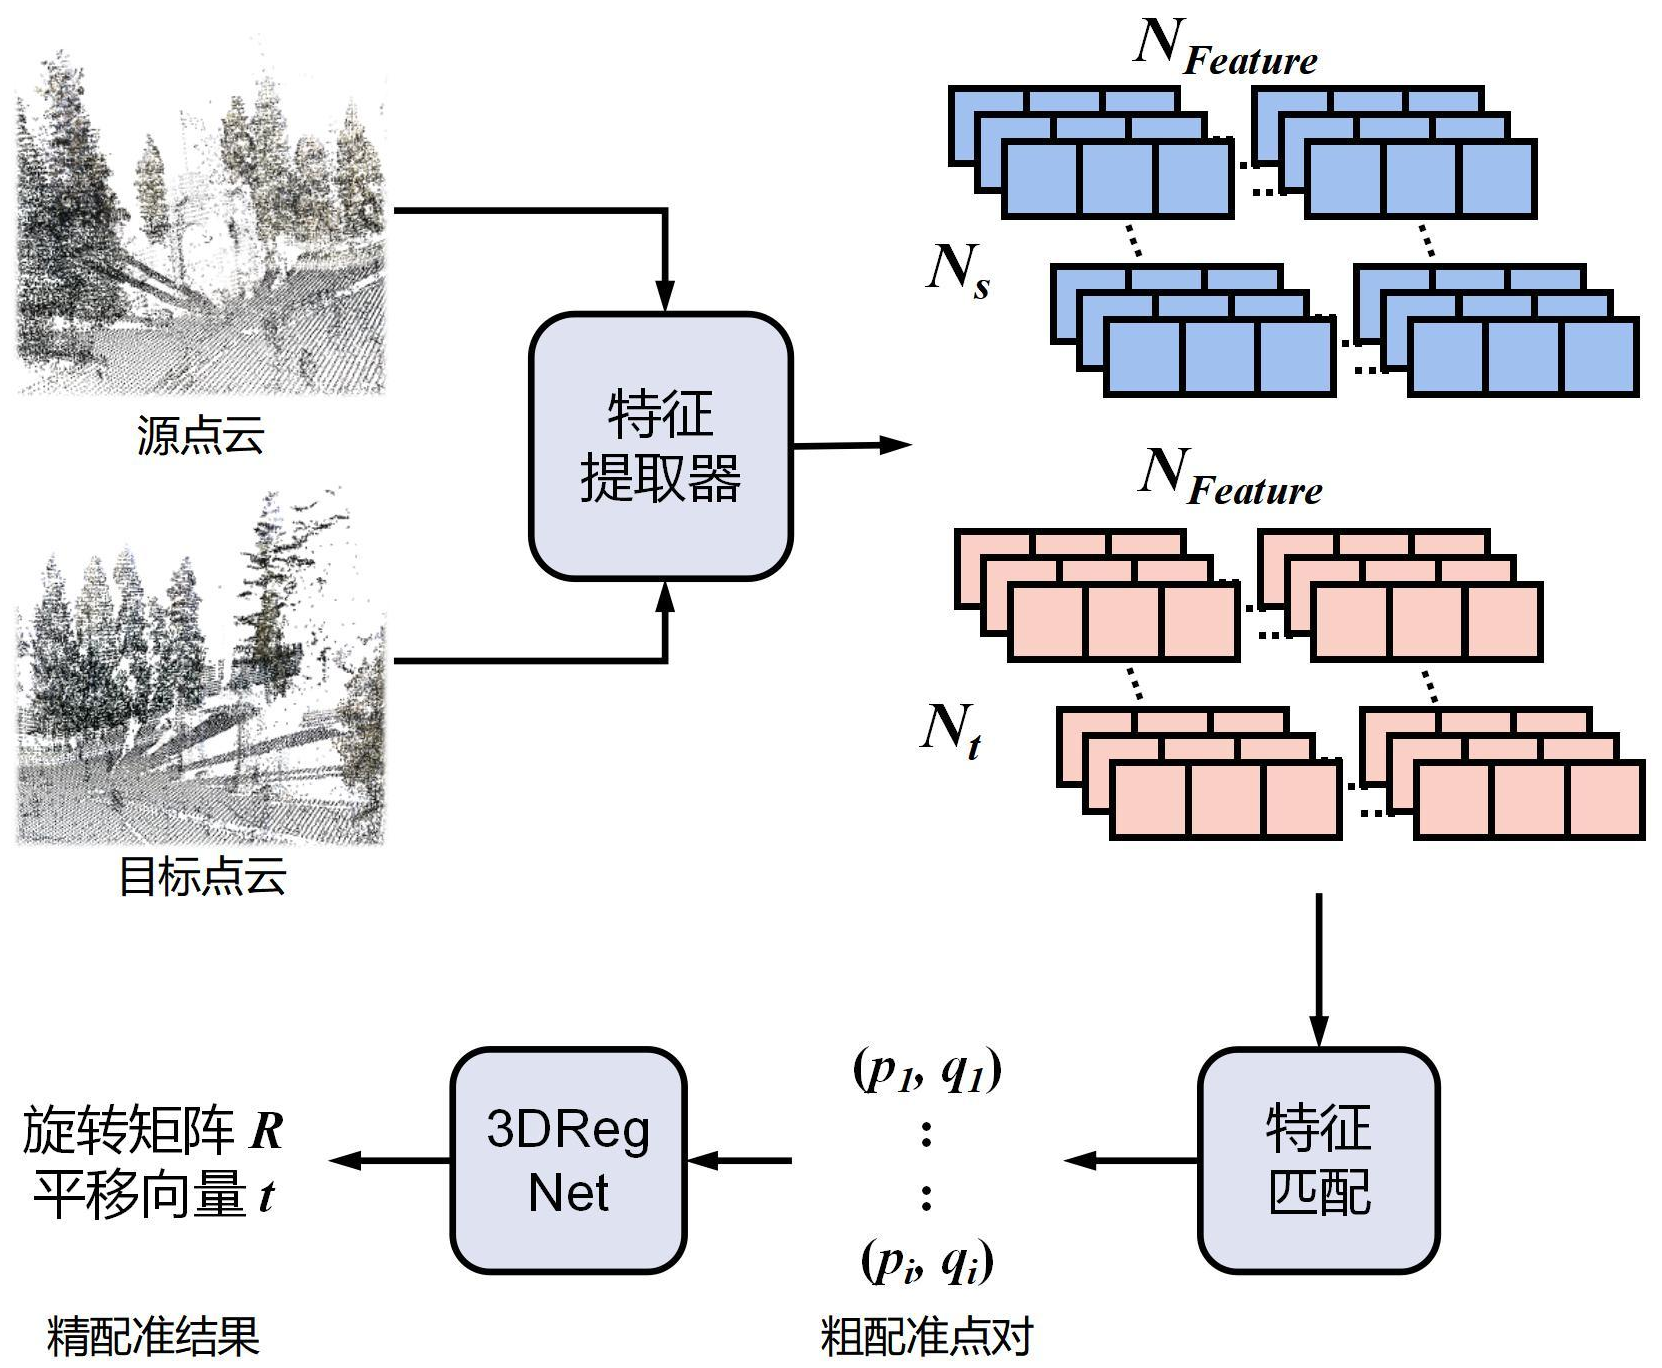
\includegraphics[width=13cm]{registration-flowchart}
	\caption{点云配准算法流程图}
	\label{registration-flowchart}
\end{figure}

\section{点云粗配准}
\subsection{局部特征描述子}
在2D图像匹配领域,寻找图像之间对应的方法是构建特征描述符,根据每个关键点及其领域的信息提取特征向量。这些基于2D图像的描述子设计给基于3D点云的描述子设计提供了思路,目前最经典的点云特征提取算法是\citet{rusu2009fast}提出的Fast Point Feature Histograms(FPFH)算法,此算法能够保证旋转不变性,同时兼顾了鲁棒性与算法效率。本章中利用了此算法提取对点云进行了特征提取。

FPFH特征在PFH特征\cite{rusu2008aligning}的基础上进行了效率优化。对于点云中的每个点(query point),选择其半径$r$范围内的$k$近邻点,这$k$个点分别与query point构成$k$个点对$(p_i,p_j)$,对于每个点对,首先构造局部坐标系:
\begin{equation}
	\left\{
	\begin{aligned}
		& u = n_i \\
		& v = (p_j-p_i) \times u \\
		& w = u \times v
	\end{aligned}
	\right.
\end{equation}

其中$n_i$表示点$p_i$处的法向量,$\times$表示外积。点对之间的角度特征用$<\alpha, \phi, \theta>$表示,定义如下:
\begin{equation}
	\left\{
	\begin{aligned}
		& \alpha = v \cdot n_j \\
		& \phi = \frac{u\cdot (p_j-p_i)}{\left\|p_j-p_i\right\|} \\
		& \theta = \arctan(w\cdot n_j, u\cdot n_j)
	\end{aligned}	
	\right.
\end{equation}


对于每个查询点的$k$个匹配对,将三个角度特征分别划分为$m$个区间,统计落在每个区间的数量分布直方图,然后将其拼接得到单个查询点的SPFH特征,其维度为$3m$,FPFH特征可以看做查询点与$k$近邻点SPFH特征的加权和
\begin{equation}
	\text{FPFH}(p_q)=\text{SPFH}(p_q)+\frac{1}{k}\sum_{i=1}^k \frac{1}{\omega_k} \cdot \text{SPFH}(p_k)
\end{equation}
其中$\omega_k$为查询点$p_q$和邻点$p_k$的距离。图~\ref{FPFH-connection}展示了每个查询点的影响区域范围,每个查询点与灰色半径范围内的$k$个点相连,查询点的FPFH特征由灰色圆圈中的$k+1$个点的SPFH直方图加权而来,其中图上标号为2的连接对FPFH特征贡献了2次。
\begin{figure}
	\centering
	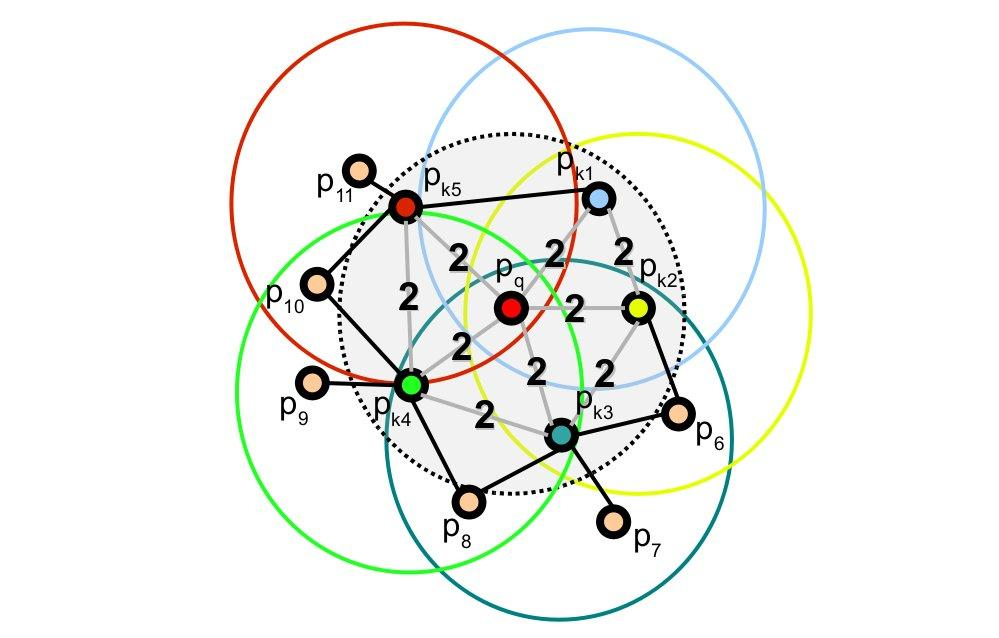
\includegraphics[width=12cm]{FPFH-connection.png}
	\caption{FPFH影响区域图}
	\label{FPFH-connection}
\end{figure}

\subsection{基于点特征的全局粗匹配}
FPFH算法能够利用点云中间的空间关系,将点用高维向量进行特征表示,这给寻找两个点云之间的点配对关系提供了工具。本章采用了KD-Tree\cite{nuchter2007cached}方式为源点云与目标点云之间建立搜索树,然后通过RANSAC方式\cite{fischler1981random}排除错误的匹配对,同时估计出两个点云之间的旋转矩阵$R$与平移向量$t$。

KD-Tree是为$k$维向量数据构建的二叉搜索树,在所有非叶子节点上用过该节点向量的超平面将$k$维空间分割成两个部分,被分割的两个子空间中的点分别作为该节点的左子树和右子树。利用KD树能够将搜索复杂度降至$O(\log n)$,提升搜索效率。

图\ref{kdtree}展示了从源点云提取特征并构造KD-Tree的示意图。树中的每一个节点为点云中各点的FPFH特征,深度为$i$的非叶子结点的分割平面为与第$i$个维度轴垂直的超平面。
\begin{figure}
	\centering
	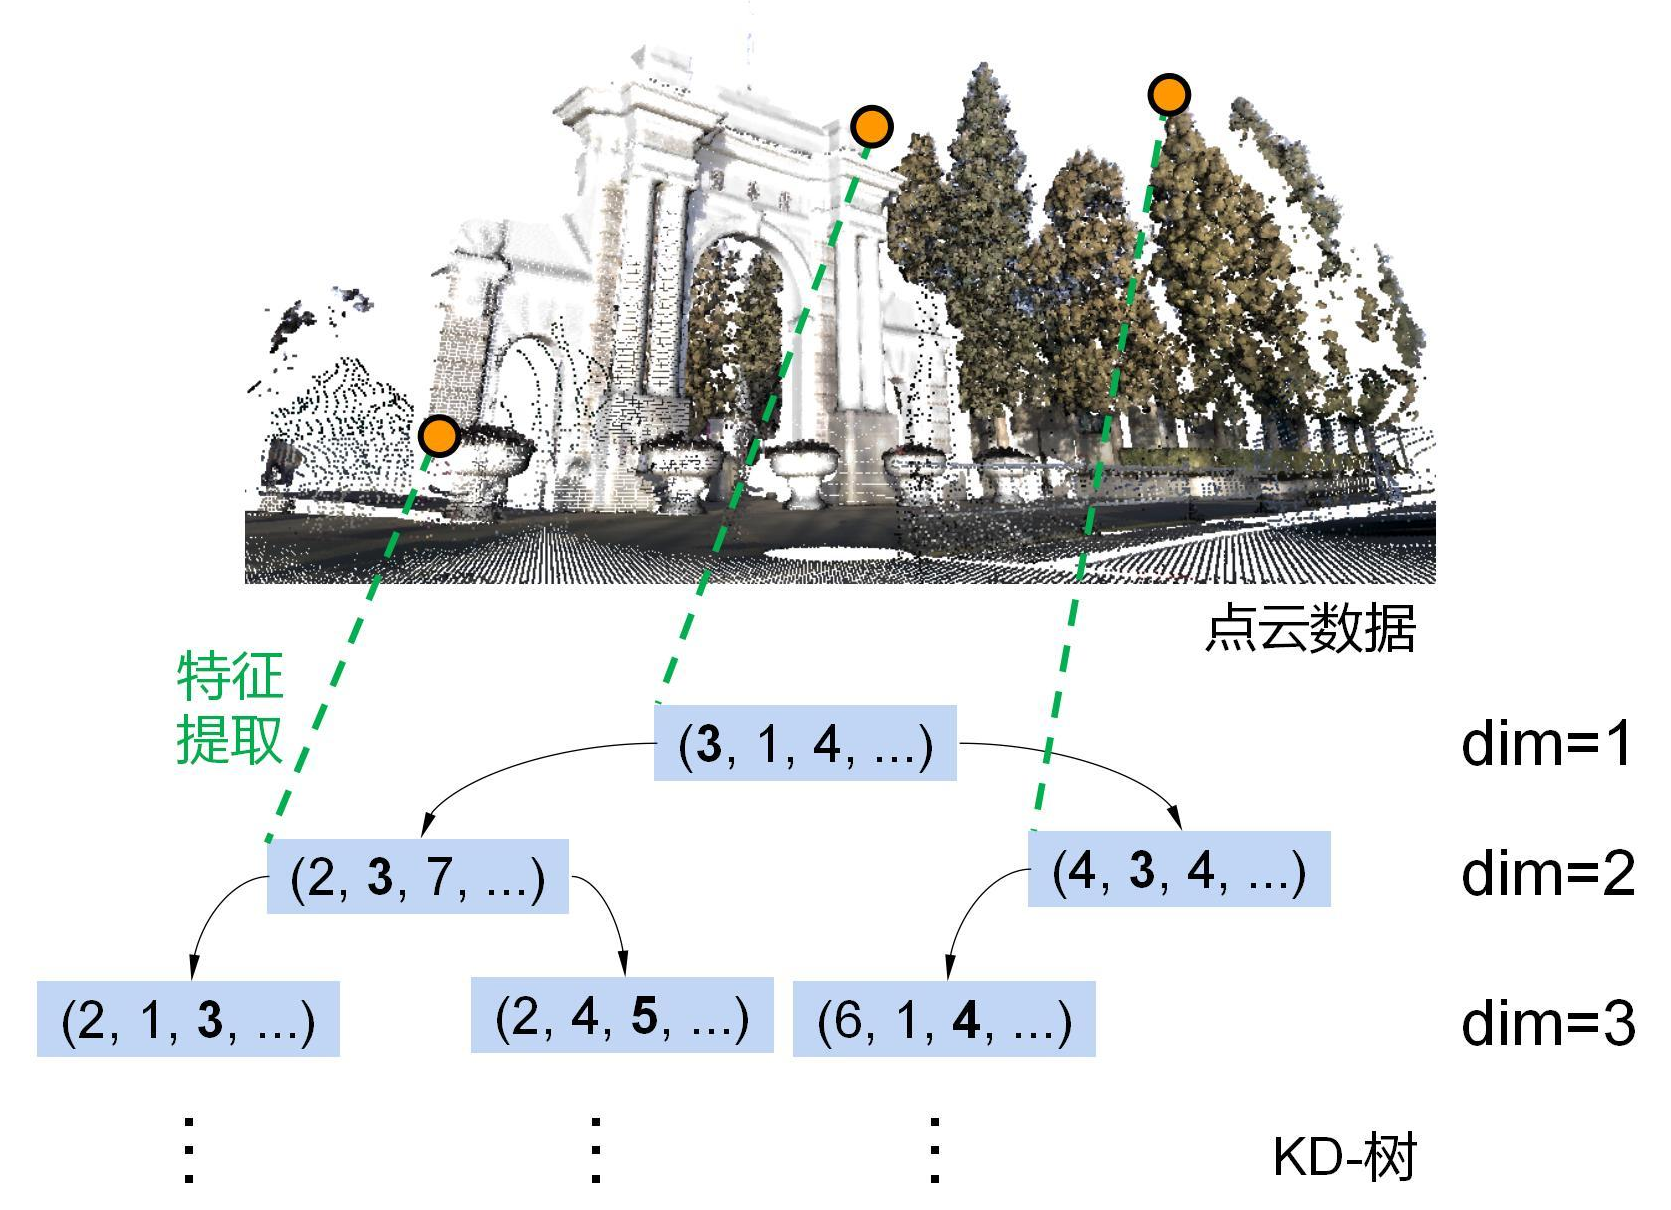
\includegraphics[width=12cm]{kdtree}
	\caption{KD树构造示意图}
	\label{kdtree}
\end{figure}

根据源点云与目标点云的FPFH特征与KD树,可以对于源点云的任意一点寻找其在目标点云中的对应,然而这样的对应并非完全准确的,在正确的配对(inlier)之外可能产生较多的错误配对(outlier)。通过RANSAC算法能够减少outlier对配准的影响,达到较好的效果。

基于RANSAC算法的点云粗配准流程如算法\ref{ransac}所示,该算法重复地从源点云中随机抽样4个点坐标,再在目标点云中根据FPFH特征寻找对应点,并利用这4个点的三维坐标估计转移矩阵$\boldsymbol{T}$,仅仅计算四个点转移矩阵是容易的,可以采用SVD分解\cite{golub1971singular}的方法来快速求得。利用转移矩阵将源点云进行变换后,判断源点云与目标点云匹配对之间的距离,统计小于给定阈值的正确匹配对(inlier)个数。在所有实验中寻找inlier个数最多的一次抽样,输出相应的转移矩阵$\boldsymbol{T}$与点对应集合$\mathcal{K}$。

\renewcommand{\algorithmicrequire}{\textbf{输入:}\unskip}
\renewcommand{\algorithmicensure}{\textbf{输出:}\unskip}
\begin{algorithm}
	\caption{基于RANSAC算法的点云粗配准}
	\label{ransac}
	\small
	\begin{algorithmic}
		\REQUIRE{一对$\boldsymbol{P}_s$, $\boldsymbol{P}_t$和FPFH特征$\boldsymbol{F}(\boldsymbol{P}_s)$, $\boldsymbol{F}(\boldsymbol{P}_t)$}
		\ENSURE{转移矩阵$\boldsymbol{T}$和点对应集合$\mathcal{K}$}
		
		\STATE{最优转移矩阵$\boldsymbol{T}_{best} \leftarrow \emptyset$}
		\STATE{最优点对应集合$\mathcal{K}_{best} \leftarrow \emptyset$}
		\STATE{max\_correspondence $\leftarrow$ 0}
		
		\FOR{$iter \leftarrow 1$ \textbf{to} $max\_iteration$}
			\STATE{从$\boldsymbol{P}_s$中随机选取4个点$(p_1, p_2, p_3, p_4)$}
			\STATE{在$\boldsymbol{P}_t$根据FPFH寻找估计对应点$(q_1, q_2, q_3, q_4)$}
			\STATE{计算能够对齐该4个点对的转移矩阵$\boldsymbol{T}$}
			\STATE{$\mathcal{K} \leftarrow \emptyset$}
			\FOR{$p_i$ \textbf{in} $\boldsymbol{P}_s$}
				\STATE{在$\boldsymbol{P}_t$中根据FPFH寻找估计对应点$q_i$}
				\IF{score($\boldsymbol{T}\cdot p_i$, $q_i$)<threshold}
					\STATE{将$p_i$, $q_i$放入$\mathcal{K}$}
				\ENDIF
				\IF{$|\mathcal{K}|$>max\_correspondence}
					\STATE{max\_correspondence $\leftarrow |\mathcal{K}|$}
					\STATE{$\mathcal{K}_{best} \leftarrow \mathcal{K}$}
					\STATE{$\boldsymbol{T}_{best} \leftarrow \boldsymbol{T}$}
				\ENDIF
			\ENDFOR
		\ENDFOR
		\RETURN{$\boldsymbol{T}_{best}$, $\mathcal{K}_{best}$}		
	\end{algorithmic}
\end{algorithm}

利用RANSAC算法,可以不必像ICP算法中依赖于两个点云的初始转移矩阵的估计。然而,由于点云中部分特征的相似重叠,同时可能存在较多的outlier,通过这一算法得到的转移矩阵并不完全精确,需要后续算法对于匹配结果进行进一步的优化。

\section{基于深度学习的点云精配准}
正如上一小节所述,尽管RANSAC算法能够减少对初始值依赖,但在性能上存在缺陷。不过RANSAC算法能够输出的两个点云的粗匹配点对与转移矩阵,这为后续的精细化提供了一个初始值。在本研究中使用3DRegNet网络排除粗匹配对中错误匹配对,并对转移矩阵进行精细化,本小节主要对该网络的结构与损失函数进行精细化。
\subsection{模型结构}
3DRegNet的网络结构如图\ref{3dregnet-structure}所示,该网络由两个子模块组成,分别是分类模块(classification block)与配准模块(registration block),前者的输入是若干对含有噪声的点匹配对,该模块对每个点对是否是inlier进行分类,并输出置信权重;后者能够直接输出从源点云到目标点之间的6DoF参数,即旋转与平移的6自由度参数。
\begin{figure}
	\centering
	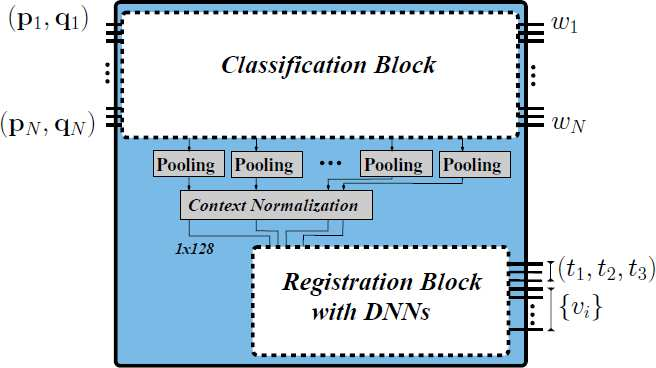
\includegraphics[width=12cm]{3dregnet-structure}
	\caption{3DRegNet网络结构图}
	\label{3dregnet-structure}
\end{figure}

分类模块结构如图\ref{3dregnet-classification}所示,$N$个3D匹配点对首先通过一个全连接层,并使用ReLU函数作为激活函数,$N$个不同的点对共享相同的权重,输出$N\times 128$维的向量。然后该输出通过$C$个连续的ResNet模块\cite{he2016deep},最后将输出通过以ReLU和tanh函数
\begin{equation}
	\text{ReLU}(x)=\max(0, x)
\end{equation}
\begin{equation}
	\tanh (x)=\frac{e^x-e^{-x}}{e^x+e^{-x}}\in (-1,1)
\end{equation}
作为激活函数的全连接层,得到$N$个匹配点对的置信权重$w_1,\cdots,w_N$。
\begin{figure}
	\centering
	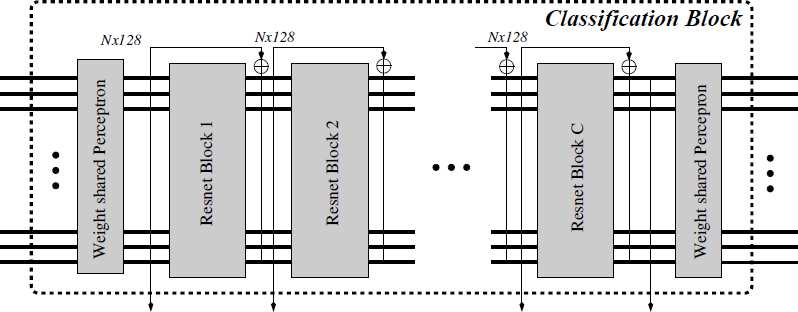
\includegraphics[width=14.5cm]{3dregnet-classification}
	\caption{3DRegNet网络分类模块}
	\label{3dregnet-classification}
\end{figure}

配准模块如图\ref{3dregnet-registration}所示,分类模块的每一层输出通过pooling提取有意义的特征,维度为$128\times 1$,总共有$C+1$个pooling层,其中提一个pooling层对应第一个ResNet模块的输入,最后一个pooling层对应最后一个ResNet模块的输出。将所有特征拼接并规范化后得到维度为$(C+1)\times 128$的特征,合并特征通过一个8通道的卷积层,卷积核大小为$3\times 3$,水平步长为1,竖直步长为2。卷积层的输出通过两个全连接层,最终得到$M+3$维的向量,其中前$M$个参数$(v_1,v_2,\cdots,v_M)$为旋转信息,后3个参数$(t_1,t_2,t_3)$为平移信息。
\begin{figure}
	\centering
	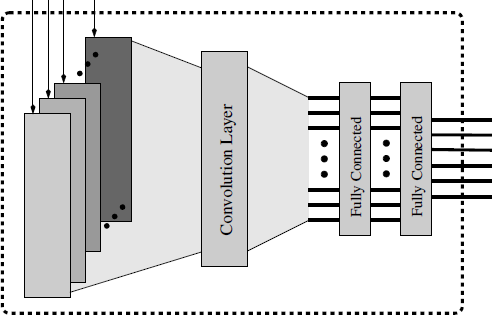
\includegraphics[width=11cm]{3dregnet-registration}
	\caption{3DRegNet网络配准模块}
	\label{3dregnet-registration}
\end{figure}

\subsection{损失函数}
3DRegNet的损失函数由两部分组成,分别是来自于分类的损失和来自配准的损失。

分类损失使用交叉熵来惩罚错误的匹配分类
\begin{equation}
	\mathcal{L}_c=\frac{1}{N}\sum_{i=1}^{N}\gamma_i H \left(y_i, \sigma(o_i)\right)
\end{equation}
其中$o_i$是配准模块在计算$w_i$时ReLU和tanh函数之前的输出,$\sigma$指sigmoid激活函数。$H(.,.)$是交叉熵函数,$y_i$是分类的ground-truth,取值为0或1,代表第$i$个匹配对是inlier还是outlier,$\gamma_i$是平衡不同对匹配点交叉熵损失的权重。

配准的损失由源点云经过变换后和目标点云对应点之间的距离得到。
\begin{equation}
	\mathcal{L}_r = \frac{1}{N}\sum_{i=1}^{N} \rho \left(\boldsymbol{q}_i, \boldsymbol{R}\boldsymbol{p}_i+\boldsymbol{t} \right)
\end{equation}
其中$\rho(.,.)$为距离度量函数,$\boldsymbol{R}$和$\boldsymbol{t}$是由网络输出的参数计算得到的转移矩阵与平移向量。

网络的总损失为
\begin{equation}
	\mathcal{L} = \alpha \mathcal{L}_c + \beta \mathcal{L}_r
\end{equation}
其中$\alpha$和$\beta$是平衡分类损失与配准损失的超参数。

\section{实验与结果}
\subsection{数据采集}
利用实验室已有的Leica激光三维扫描仪设备,本实验首先在清华二校门和客厅分别进行了点云数据采集,分别代表了在三维重建中的室外大场景环境与室内环境,其中客厅场景是封闭的,面积约为\SI{30}{m^2}左右。在每个场景中选择了三个不同的位置,将扫描仪设为中等精度进行扫描,其扫描点云详情如表\ref{blk360-data}所示。

\begin{table}
	\centering
	\caption{扫描点云数据}
	\label{blk360-data}
	\begin{tabular}{cccc}
		\toprule
		扫描编号 & 场景 & 点数量 & 文件大小 \\
		\midrule
		1 & 室内 & 11686747 & 568.78MB \\
		2 & 室内 & 12319474 & 599.61MB \\
		3 & 室内 & 10272879 & 500.20MB \\
		4 & 室外 & 6382625  & 309.88MB \\
		5 & 室外 & 6284718  & 308.37MB \\
		6 & 室外 & 9435253  & 460.13MB \\
		\bottomrule
	\end{tabular}
\end{table}

图\ref{registration-data}展示了以上两个场景的点云数据。其中图\ref{sub-indoors}和图\ref{sub-outdoors}分别是测站1和测站4的数据预览图。
\begin{figure}
	\centering
	\subcaptionbox{室内环境\label{sub-indoors}}
	{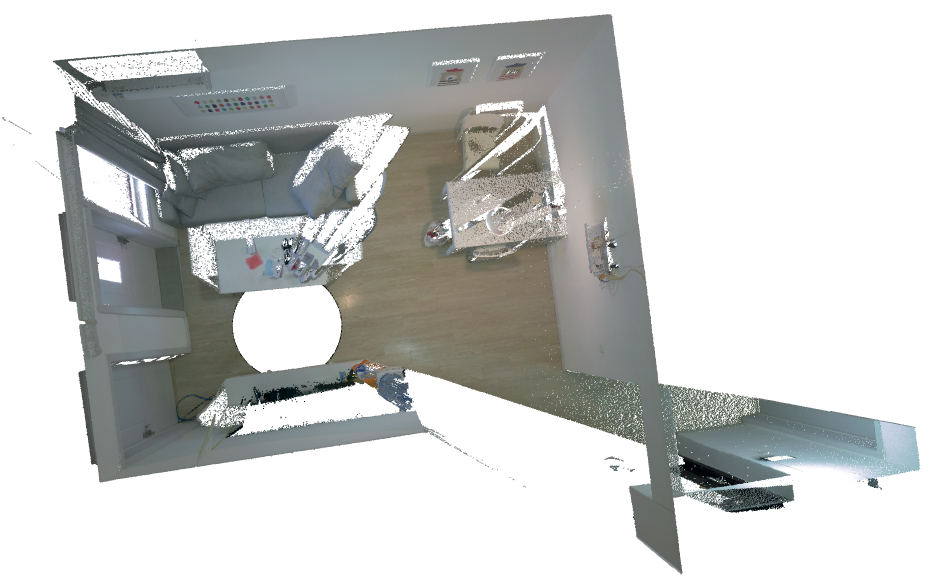
\includegraphics[width=12cm]{data-indoors}}\\
	\subcaptionbox{室外环境\label{sub-outdoors}}
	{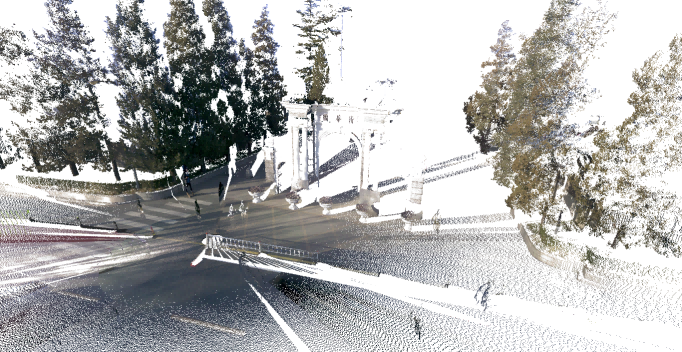
\includegraphics[width=12cm]{data-outdoors}}
	\caption{实验数据预览}
	\label{registration-data}
\end{figure}

\subsection{全局点云配准实验}
\label{global-registration-experiment}
在这一小节中,本文基于上述coarse-to-fine的点云配准框架,试图采用增量式重建的方法对多点云进行融合,生成场景的三维模型,即首先从所有点云数据中选择两个点云作为源点云和目标点云进行配准,然后将配准后的点云看做目标点云,再选择一帧新的点云数据作为源点云,估计转移矩阵,重复进行上述操作直至所有点云之间都被有效地配准,完成场景重建。

以室外场景重建为例,接下来介绍在本次算法实验中一些参数的选择。在RANSAC粗配准中,本文采用了两种剪枝算法,来提早对错误匹配进行过滤,第一个是检查两个点云的距离是否小于0.2,第二是在源点云和目标点云随机选择两对对应点连线,检查$\|\text{edge}_{src}\|>0.9*\|\text{edge}_{tar}\|$和$\|\text{edge}_{tar}\|>0.9*\|\text{edge}_{src}\|$是否成立。根据\citet{choi2015robust}提供的经验,本文将RANSAC算法中的最大迭代次数和最大验证次数设为4000000和500。对于3DRegNet网络,本研究利用了作者提供的预训练模型,该模型在ICL-NUIM数据集和SUN3D数据集\cite{zhou2014learning}上进行训练,前者包括了4个不同的场景共25000个不同的匹配点对,后者包括了13个场景共3700个匹配点对。在3DRegNet网络中,设置$C=8$,损失函数中分类和配准的平衡系数分别为$\alpha=0.5, \beta=10^{-3}$。

首先选择扫描4和扫描5的点云进行配准。这两个点云的初始位置如图\ref{reg-init}所示,分别在二校门南侧的左右两边扫描得到,以大小为0.3的体素对点云进行降采样后得到的结果如图\ref{reg-downsample},为了更直观的显示,这里将原始扫描中的颜色信息去除,并将测站4设为红色,测站5设为蓝色;下一步对点云进行法线估计与FPFH特征值计算,点云法线信息如图\ref{reg-normal}所示,箭头方向为该点处的法线向量;经过RANSAC粗配准后,结果如图\ref{reg-ransac}所示,两个点云被较好地对齐,但部分地方的效果依旧不够理想,同时粗配准也能够对两个点云中的点进行粗配对,配对结果如图\ref{reg-correspondence}所示,这里随机选择了500对匹配对,并用绿线相连接;将匹配对输入3DRegNet网络,得到最终转移矩阵的估计值,将此转移矩阵作用在降采样之前的点云上,其配准结果如图\ref{reg-refine}所示。
\begin{figure}
	\centering
	\subcaptionbox{初始点云\label{reg-init}}
	{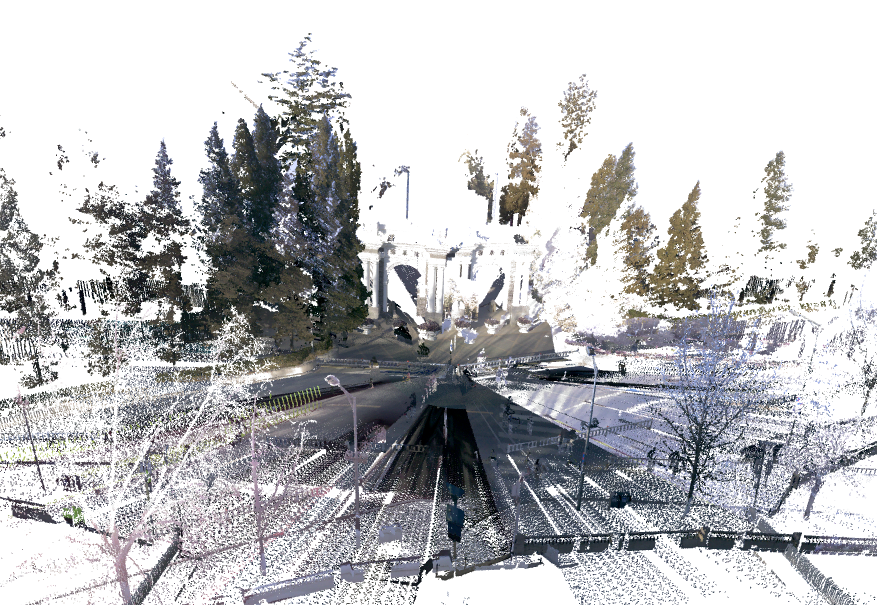
\includegraphics[width=7cm]{reg-init}}
	\subcaptionbox{降采样点云\label{reg-downsample}}
	{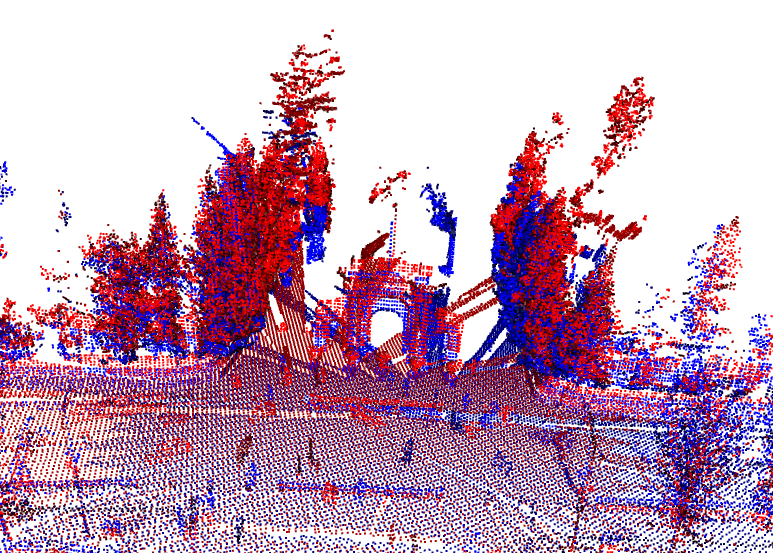
\includegraphics[width=7cm]{reg-downsample}}\\
	\subcaptionbox{法线估计\label{reg-normal}}
	{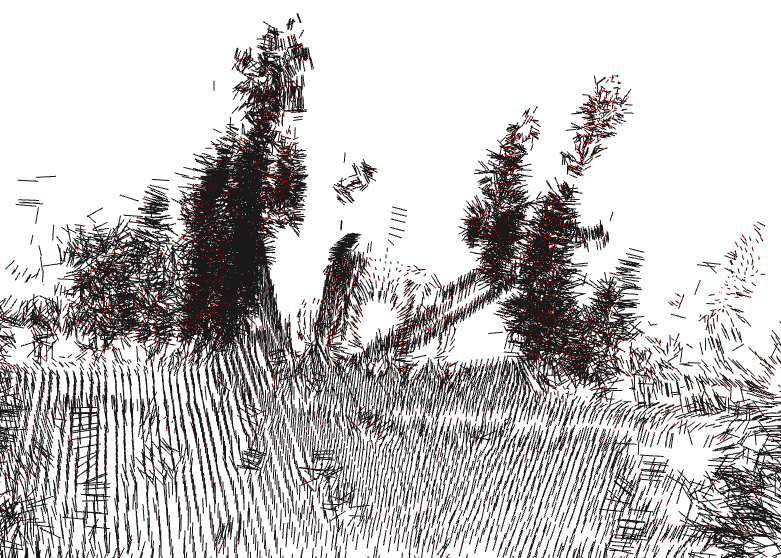
\includegraphics[width=7cm]{reg-normal}}
	\subcaptionbox{粗配准\label{reg-ransac}}
	{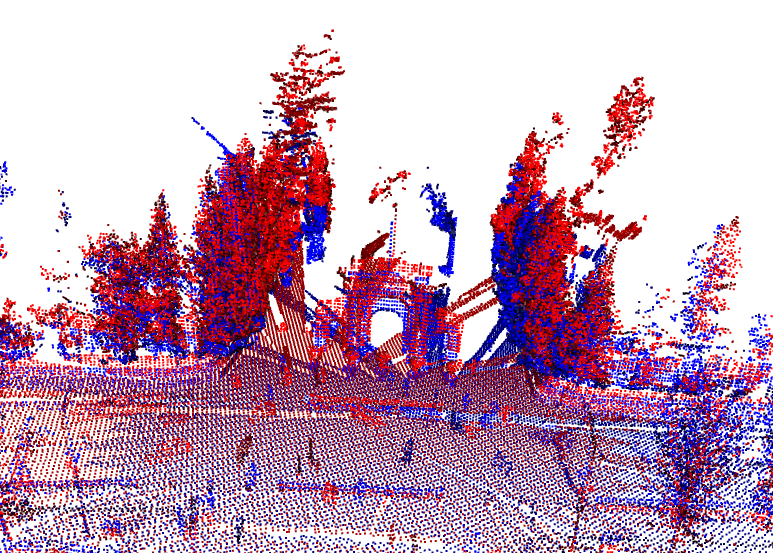
\includegraphics[width=7cm]{reg-ransac}}\\
	\subcaptionbox{点对估计\label{reg-correspondence}}
	{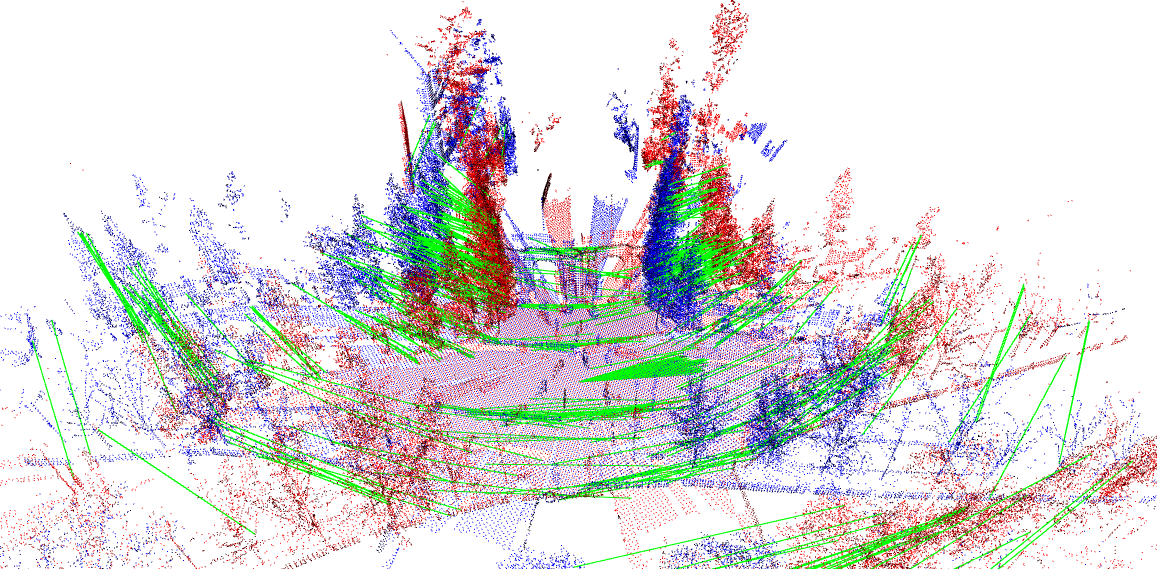
\includegraphics[width=7cm]{reg-correspondence}}
	\subcaptionbox{精配准结果\label{reg-refine}}
	{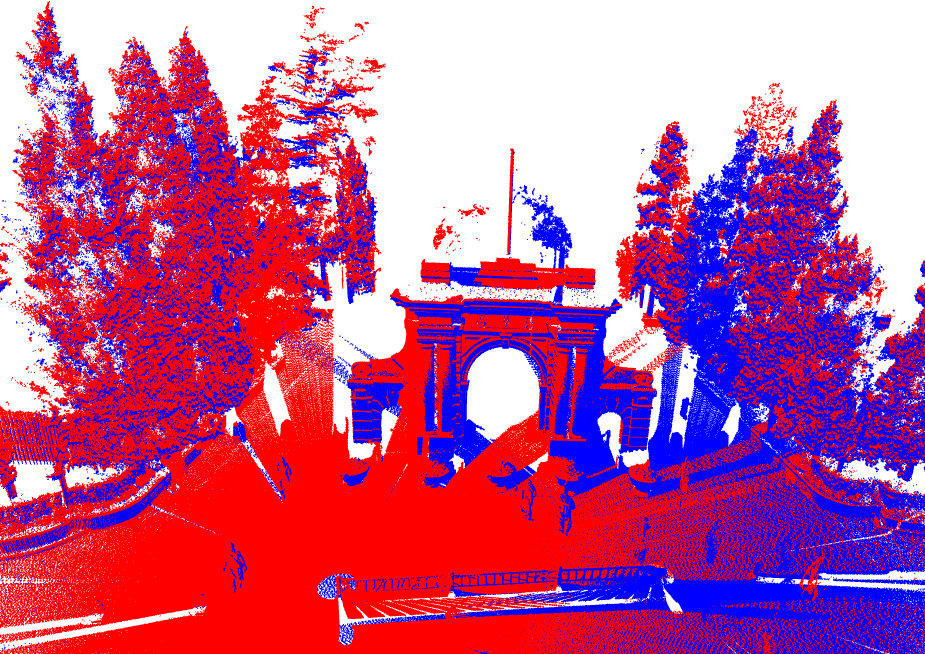
\includegraphics[width=7cm]{reg-refine}}
	\caption{双点云融合过程及结果}
	\label{reg-outdoor-process}
\end{figure}

利用上述双点云融合的过程对多个点云数据进行融合,得到结果如图\ref{reg-result}所示,其中图\ref{reg-result-outdoor}是二校门场景的重建结果,图\ref{reg-result-indoor}是客厅场景的重建结果,两个场景中的三个点云分别用红色、绿色和蓝色进行了标记。从主观上来看,不同位置扫描得到的点云融合效果较好。
\begin{figure}
	\centering
	\subcaptionbox{二校门场景\label{reg-result-outdoor}}
	{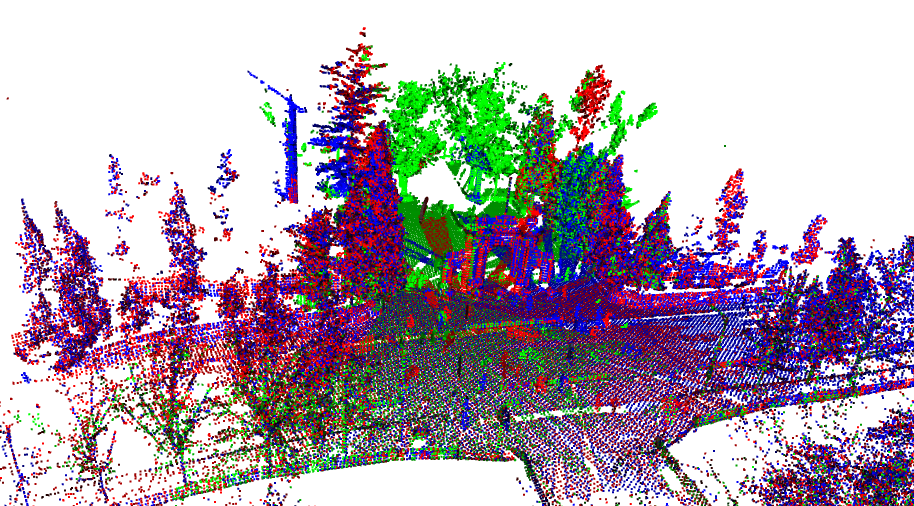
\includegraphics[width=14cm]{reg-outdoor-overall}}\\
	\subcaptionbox{客厅场景\label{reg-result-indoor}}
	{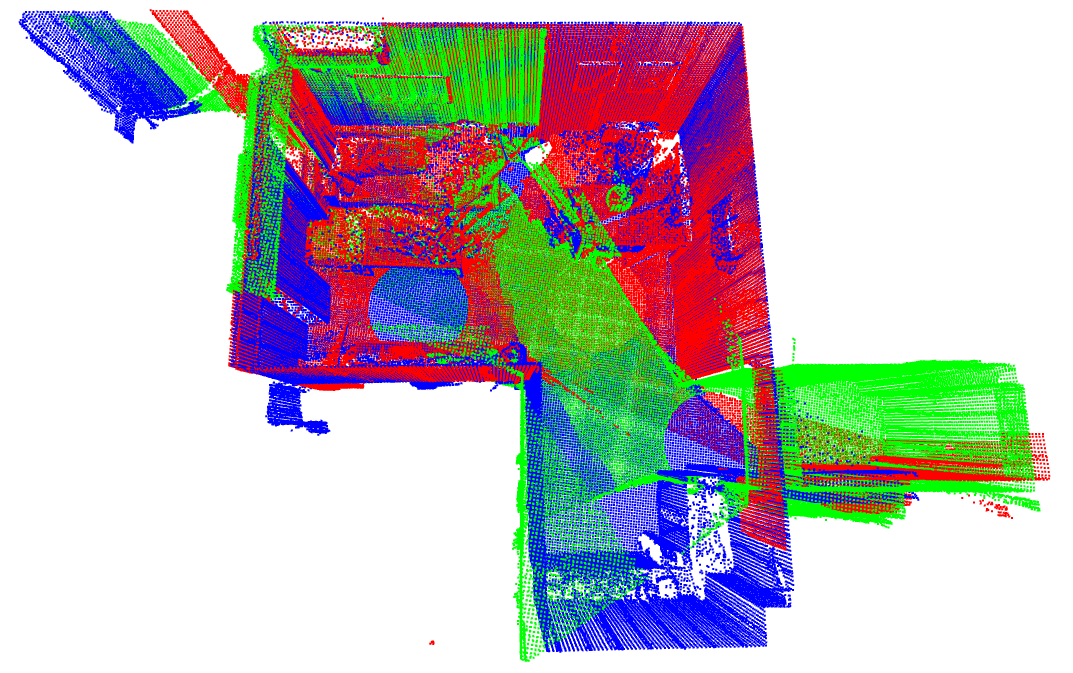
\includegraphics[width=14cm]{reg-indoor-overall}}
	\caption{多点云融合结果}
	\label{reg-result}
\end{figure}

\subsection{算法评价}
不同点位测量的局部点云结果的配准结果能够直观地评判,但缺少客观的评价指标。因此,为了能准确评估点云配准的算法性能,为估计结果提供ground-truth参照,本文采用人工变换的方式,对同一点位测量的点云中进行采样和处理,并提供随机的旋转和平移,得到目标点云,通过比较若干种点云配准算法的结果与ground-truth之间的差异,来说明本文介绍的算法的有效性。

以表\ref{blk360-data}中测站4的数据作为对象,本实验采用4种不同的方式来生成源点云与目标点云。在第一组实验中,源点云由从扫描点云中直接随机采样的20000个点构成,并给予随机旋转和平移得到目标点云,即源点云与目标点云中的每个点都存在着一一对应的关系;在第二组实验中,源点云和目标点云为扫描点云中分别采样的20000个点,并给予目标点云随机旋转和平移;在第三组实验中,先按照第一组的方式生成源点云与目标点云,然后对目标点云中的每个点的每个维度坐标,加入了均值为0,方差为0.01的高斯噪声,模拟数据采样中存在的噪声情况;在第四组实验中,整体点云被分割成三个相连的子空间$\boldsymbol{P} = \{\mathcal{P}_1, \mathcal{P}_2, \mathcal{P}_3\}$,源点云从$\{\mathcal{P}_1, \mathcal{P}_2\}$中采样20000个点,目标点云从$\{\mathcal{P}_2, \mathcal{P}_3\}$中采样20000个点,并给予随机旋转和平移,该组实验模拟两个点云之间只存在部分匹配(partial-to-partial)的情况。

在本实验中,采用了三种点云配准方法,分别为经典的ICP算法(初始旋转矩阵为单位阵,平移向量为零向量)、FPFH+RANSAC(即仅进行粗配准),以及本文提到的coarse-to-fine的配准方法。所有点云处理前先进行了归一化操作,在随机变换步骤中,每个轴旋转角度$\phi, \theta, \psi$从$[-45^\circ, 45^\circ]$中均匀随机采样得到,每个轴向平移距离值$t_1, t_2, t_3$从$[-0.5, 0.5]$中均匀随机采样得到,旋转矩阵可以表示为
\begin{align}
	\boldsymbol{R} & = 
	\begin{bmatrix}
		1 & 0 & 0 \\
		0 & \cos\phi & -\sin\phi\\
		0 & \sin\phi & \cos\phi
	\end{bmatrix}
	\begin{bmatrix}
		\cos\theta & 0 & \sin\theta\\
		0 & 1 & 0 \\
		-\sin\theta & 0 & \cos\theta
	\end{bmatrix}
	\begin{bmatrix}
		\cos\psi & -\sin\psi & 0\\
		\sin\psi & \cos\psi & 0 \\
		0 & 0 & 1
	\end{bmatrix}\\
	 & = 
 	\begin{bmatrix}
 		\cos\theta\cos\phi &  \sin\psi\sin\theta\cos\phi-\cos\psi\sin\phi & \cos\psi\sin\theta\cos\phi+\sin\psi\sin\phi \\
 		\cos\theta\sin\phi & \sin\psi\sin\theta\sin\phi+\cos\psi\cos\phi & \cos\psi\sin\theta\sin\phi-\sin\psi\cos\phi \\
 		-\sin\theta & \sin\psi\cos\theta & \cos\psi\cos\theta
 	\end{bmatrix}
\end{align}

平移矩阵为
\begin{equation}
	\boldsymbol{t} = (t_1, t_2, t_3)
\end{equation}

配准结果如图\ref{reg-indoor-exp}所示,分别展示了四组实验下三种不同方法的结果及其与Ground truth的对比,为了更好地展示匹配效果,此处将原始点云中的彩色数据替换为了统一的颜色,源点云被标记为红色,目标点云被标记为蓝色。图\ref{reg-indoor-exp1}对应了第一组两个完全相同点云的情况,此时ICP算法陷入了局部最优,没有很好地配准两个点云,而RANSAC算法能够较好粗对齐二者,并在通过3DRegNet网络后达到几乎完美的匹配,需要注意的是,在这组实验中由于配准后两个点云的点会完全重合,因此在RANSAC+3DRegNet和Ground truth图像中只能看到红色点云的部分,这一结果也能证明本文算法的有效性。图\ref{reg-indoor-exp2}和图\ref{reg-indoor-exp3}分别对应重复采样的点云和含噪声的点云的情况,从直观上来看,ICP算法和本文算法都能够很好地完成配准,并且两者看不出差异。图\ref{reg-indoor-exp4}对应这部分重合点云配准实验,在这一组实验中,ICP算法无法找到最优解,因为源点云中大多数点无法在目标点云中找到对应,而RANSAC算法的对齐效果虽然不够完美,但也给3DRegNet网络提供了一个较好的初值,而精配准后的结果效果直观上较好,与Ground truth较为接近。

\begin{figure}
	\centering
	\subcaptionbox{完全相同点云\label{reg-indoor-exp1}}
	{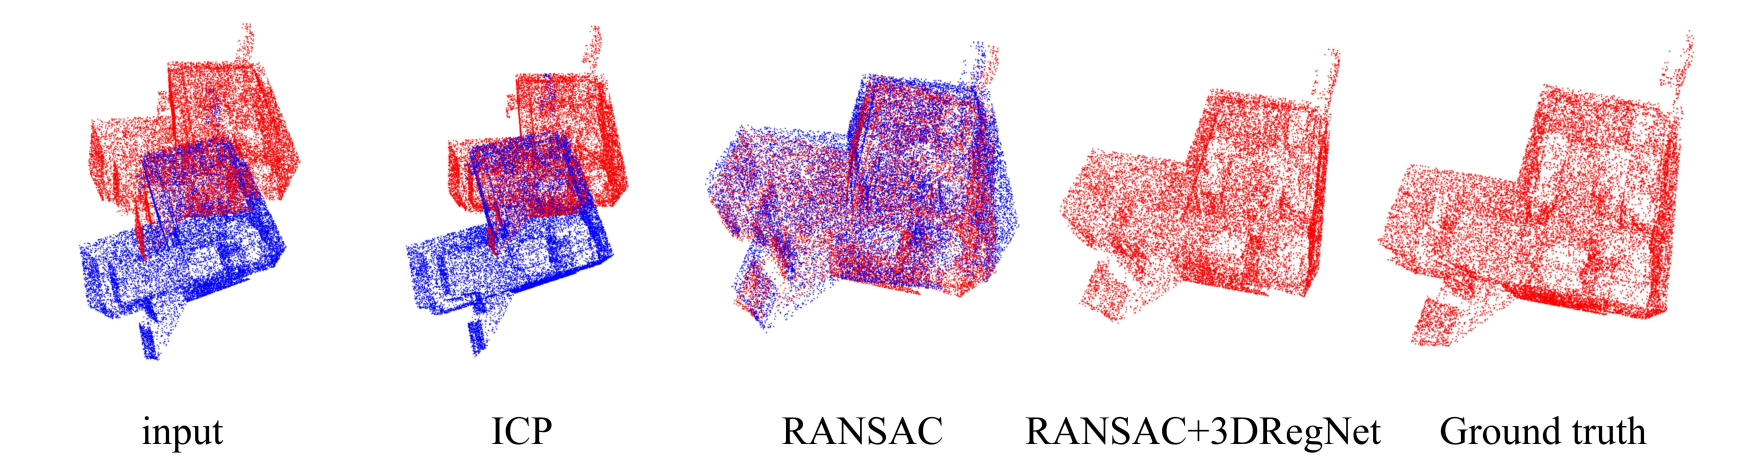
\includegraphics[width=15cm]{reg-indoor-exp1}}\\
	\subcaptionbox{重复采样点云\label{reg-indoor-exp2}}
	{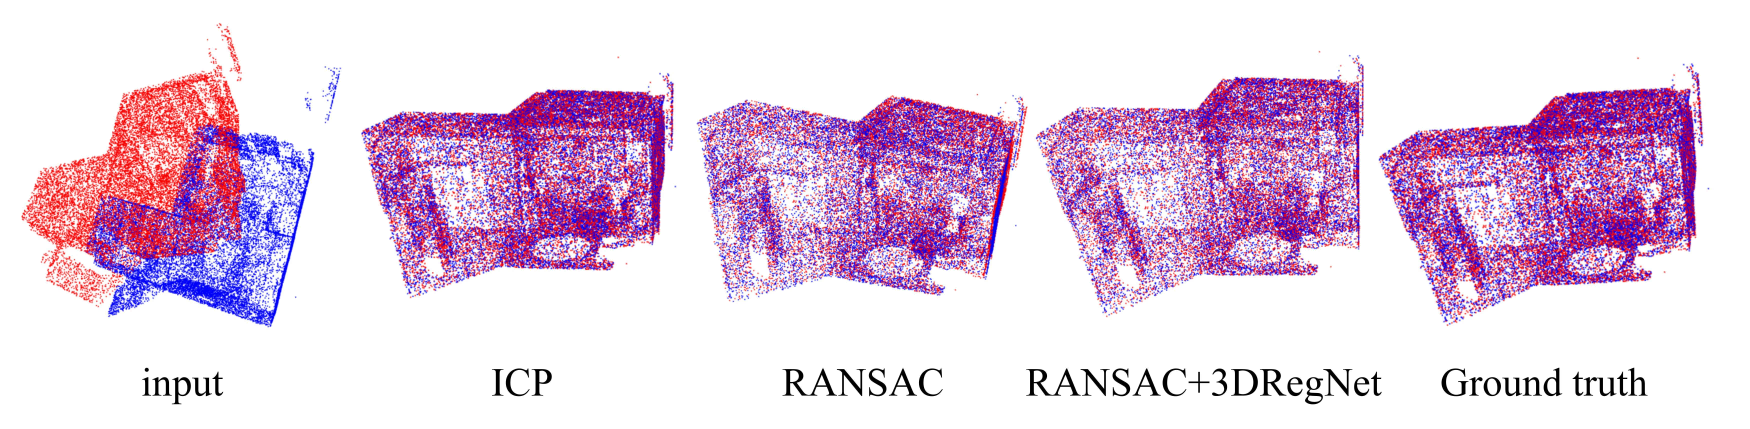
\includegraphics[width=15cm]{reg-indoor-exp2}}\\
	\subcaptionbox{含噪声点云\label{reg-indoor-exp3}}
	{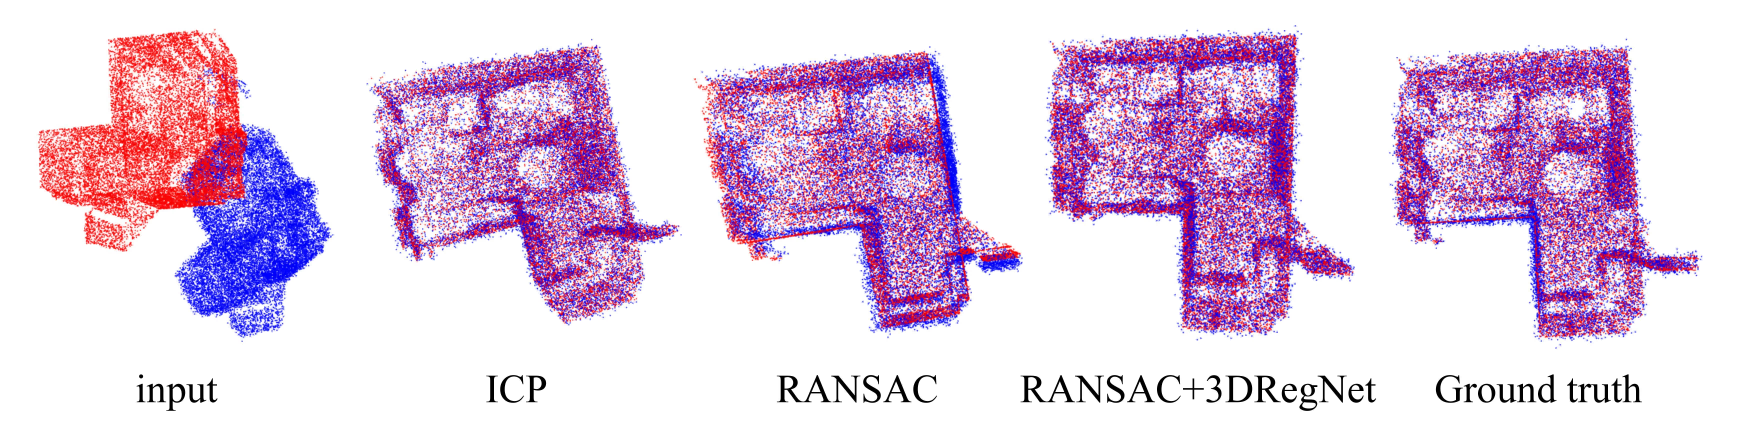
\includegraphics[width=15cm]{reg-indoor-exp3}}\\
	\subcaptionbox{部分重合点云\label{reg-indoor-exp4}}
	{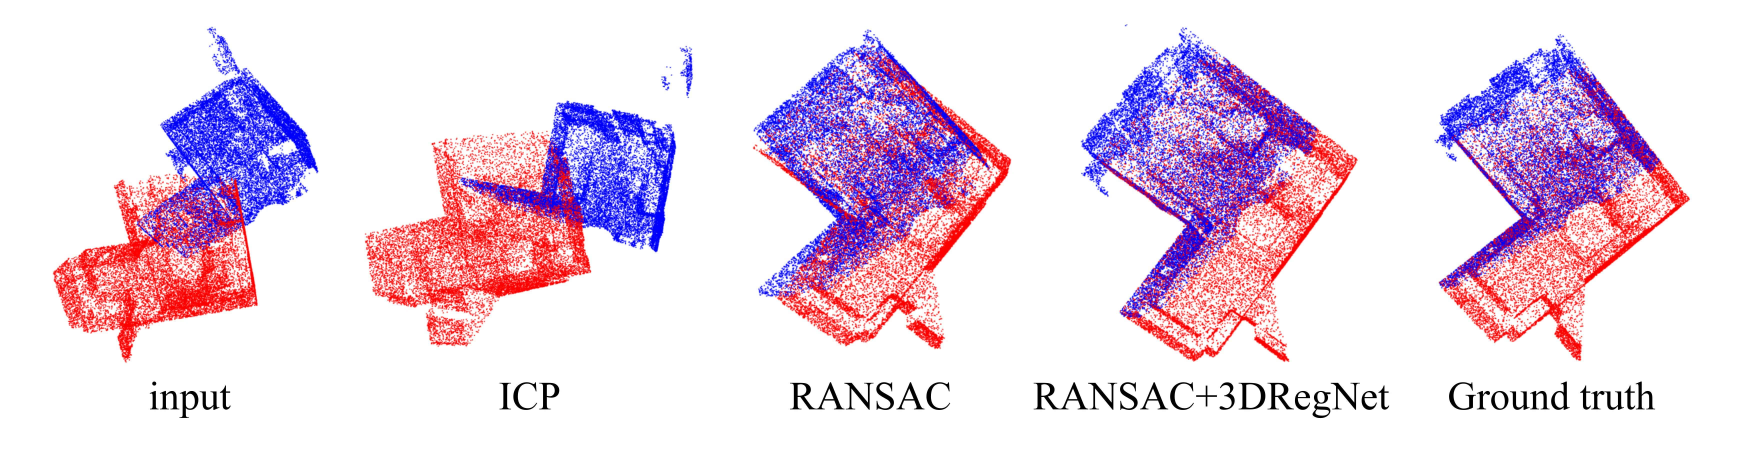
\includegraphics[width=15cm]{reg-indoor-exp4}}\\
	\caption{室内扫描点云配准实验结果}
	\label{reg-indoor-exp}
\end{figure}

对于点云配准精度的评价,主要是计算估计的旋转矩阵和平移向量与真实旋转矩阵和平移向量之间的距离。目前最常用的度量是平均相对角度误差(Mean Relative Angular Error, MRAE)和平均相对平移误差(Mean Relative Translation Error, MRTE),除此之外还有均方误差MSE,绝对平均误差MAE等。本文选用MRAE和MRTE来评价本文算法,两者的计算如下
\begin{equation}
	\label{mrae}
	\text{MRAE} = \frac{1}{N}\sum_{i=1}^N \arccos \frac{\text{tr}({\boldsymbol{R}_{pre}^i}^{-1}\boldsymbol{R}_{gt}^i)-1}{2}
\end{equation}
\begin{equation}
	\label{mrte}
	\text{MRTE} = \frac{1}{N}\sum_{i=1}^N \| \boldsymbol{t}_{pre}^i - \boldsymbol{t}_{gt}^i\|_2
\end{equation}
其中$\boldsymbol{R}_{pre}^i$和$\boldsymbol{t}_{pre}^i$表示第$i$次配准实验的预测旋转矩阵和平移向量,$\boldsymbol{R}_{gt}^i$和$\boldsymbol{t}_{gt}^i$表示第$i$次实验的真实旋转矩阵和向量。MRAE的单位是角度,MRTE的单位是长度,根据表达式\ref{mrae}和\ref{mrte}可得,若预测的$\boldsymbol{R}$和$\boldsymbol{t}$与真实值越接近,则两个评价指标越接近于0,表示配准的效果越好。

本文在室内和室外的两个扫描点云上分别对四组实验进行了10次重复实验,每次采样的点和转移矩阵均为随机生成,分别计算这10次实验的MRAE和MRTE指标的平均值,结果分别如表\ref{indoor-evaluate}和表\ref{outdoor-evaluate}所示。

\begin{table}
	\centering
	\caption{室内扫描点云配准结果评价}
	\label{indoor-evaluate}
	\begin{tabular}{ccccccc}
		\toprule
		\textbf{} & \multicolumn{3}{c}{\textbf{MRAE}}                 & \multicolumn{3}{c}{\textbf{MRTE}}                \\
		& \textbf{ICP} & \textbf{RANSAC} & \textbf{Ours}    & \textbf{ICP} & \textbf{RANSAC} & \textbf{Ours}   \\ \midrule
		完全相同点云    & 26.1960      & 9.9024          & \textbf{0.0000}  & 0.3867       & 0.0337          & \textbf{0.0000} \\
		重复采样点云    & 24.8931      & 6.5319          & \textbf{0.0164}  & 0.3083       & 0.0180          & \textbf{0.0001} \\
		含噪声点云     & 20.2065      & 21.8961         & \textbf{14.7626} & 0.3061       & 0.0771          & \textbf{0.0410} \\
		部分重叠点云    & 41.0603      & 37.7057         & \textbf{31.4172} & 0.3169       & 0.1382          & \textbf{0.1132} \\ \bottomrule
	\end{tabular}
\end{table}

\begin{table}
	\centering
	\caption{室外扫描点云配准结果评价}
	\label{outdoor-evaluate}
	\begin{tabular}{ccccccc}
		\toprule
		\textbf{} & \multicolumn{3}{c}{\textbf{MRAE}}                 & \multicolumn{3}{c}{\textbf{MRTE}}                \\
		& \textbf{ICP} & \textbf{RANSAC} & \textbf{Ours}    & \textbf{ICP} & \textbf{RANSAC} & \textbf{Ours}   \\ \midrule
		完全相同点云    & 54.6477          & 7.3719          & \textbf{0.0000} & 0.5774       & 0.01359         & \textbf{0.0000} \\
		重复采样点云    & 67.8208          & 7.8853          & \textbf{0.1622} & 0.5998       & 0.0113          & \textbf{0.0002} \\
		含噪声点云     & \textbf{33.0697} & 49.0816         & 36.0937         & 0.3102       & 0.0376          & \textbf{0.0124} \\
		部分重叠点云    & 52.7475          & 14.6118         & \textbf{0.1655} & 0.3968       & 0.0105          & \textbf{0.0001} \\ \bottomrule
	\end{tabular}
\end{table}

从表\ref{outdoor-evaluate}中可得,由于给予ICP算法的初值是单位矩阵,因此算法常常会收敛到错误的局部极小值,因此角度和位移误差都很大,而经过RANSAC能够很好的估计出平移向量$\boldsymbol{t}$,因此首先能够使MRTE减小,进一步通过3DRegNet网络的精配准,使误差进一步缩小。另一方面,从四个实验组来看,不管采用何种方法,其匹配误差满足:完全相同的点云<重复采样点云<含噪声点云<部分重叠点云,而后两种情况更加接近真实数据采集的情况,同时本文的算法在这两组实验中的表现较好,因此在处理真实扫描数据中能够获得比传统方法更好的配准效果。

\section{本章小结}
本章结合传统点云配准方法和深度学习方法,提出了一种新的点云配准流程,该方法能够不依赖于点云的初始转移矩阵的估计,首先从点云中估计粗匹配对,然后再利用3DRegNet对匹配结果进行精细化调整。

同时,本章通过对在室内和室外分别采集的数据进行了实验,利用上述点云配准方法完成了场景构建并对该算法性能进行了评价。







